\documentclass[12pt]{article}
\usepackage[utf8]{inputenc}
\usepackage[english, main=bulgarian]{babel}
\usepackage{hyperref}
\usepackage{url}
\usepackage{graphicx}
\usepackage{geometry}
\geometry{left=3cm,right=1cm,top=1cm,bottom=3cm}
\usepackage{xcolor}
\usepackage{tikz}
\usetikzlibrary{trees}
\usepackage{tabularx}
\hypersetup{
	colorlinks,
	linkcolor={black},
	citecolor={black},
	urlcolor={black}
}
\usepackage{setspace}

\renewcommand{\baselinestretch}{1.5} 

\begin{document}
	\selectlanguage{bulgarian}
	\tableofcontents
	\newpage
	\begin{abstract}
		Целта на проекта е създаване на образователно-информационна платформа, пряко свързана с ИТ сферата.\\\\
		Образователната част се състой в излагане на изучавания материал чрез кратки тематични видео уроци, теоретични въпроси и тестове и решаване на много различни по сложност практически задачи. Видео уроците са представени и ще се допълват и актуализират от професионалисти в тази дейност като учители по информатика, ръководители на школи, научни дейци, известни национални състезатели и други.\\\\
		Информационната част съдържа:
		\begin{itemize}
			\item новини за събития, свързани с програмирането, като състезания (национални, международни, онлайн и други), курсове, семинари, работилници (Workshops) и конференции;
			\item кратко представяне под формата на визитки на лекторите и фирми от ИТ сферата с описание на тяхната дейност и постижения
		\end{itemize}
		Тестовата част съдържа задачи за упражнение и проверка на знания(домашни и изпити), които биват автоматично оценявани.\\\\
		Целта е ползвателите да добият по-пълна представа за софтуерното инжинерство и да се даде възможност за популяризация на дейности и мероприятия на фирми от индустрията за обучаване на необходимите им кадри.
	\end{abstract}
	\newpage
	\section{Сравнение}
	\subsection{Обучителни системи}
	Нашата обучителни системи съдържа:
	\begin{itemize}
	  \item Видео уроци и информация за лектора
	  \item Публична дискусия към всеки урок
	  \item Секция „Новини“ с информация за събития, свързани с информатиката и информационните технологии
	  \item Секция с типични шеги за програмисти, с които все може да се посмее за почивка
	\end{itemize}
	\subsubsection{Уча.се}
	В Уча.се има уроци по програмиране, но те са просто нарязани 4-часови видео от архивите на СофтУни, липсват практически и дори липсват теоретични задачи. Освен това базата е не задоволителна, накъсана и на моменти хаотична.
	\begin{table}[ht]
		\centering
		\resizebox{\textwidth}{!}
		{
			\begin{tabular}{l|l|l}
				\bf{Критерии} & \bf{Уча.се} & \bf{Този проект (TechEdu ++)}\\
				\hline
				\bf{Продължителност на уроците} & 9-10 мин & от 10 мин до 20 мин \\
				\hline
				\bf{Теоретични тестове} & Не & изготвят се за всеки урок\\
				\hline
				\bf{Практически задачи} & Не & има и то различни трудности,\\
				& & включват се и задачи от различни \\
				& & състезания (национални, международни и онлайн)\\
				\hline
				\bf{Комуникация} & има коментари по всяко видео & има специализирана система,\\
				& и те често са изпълнени със спам & която представлява чат със стаи \\
				& & и служи за подобряване\\
				& & на комуникацията\\
				\hline
			\end{tabular}
		}
	\end{table}\\
	\subsubsection{Telerik Academy / SoftUni}
	Има уроци по програмиране, но те са твърде дълги - 4 часа, а някои стигат до 6. Освен това имат няколко несинхронизирани системи, което е неудобно за учениците.
	\begin{table}[ht]
	\centering
	\resizebox{\textwidth}{!}
	{
		\begin{tabular}{l|l|l}
			\bf{Критерии} & \bf{Telerik Academy / SoftUni} & \bf{Този проект (TechEdu ++)}\\
			\hline
			\bf{Продължителност на уроците} & 4-5-6 часа & от 10 мин до 20 мин\\
			&(уроците са предназначени за&(тематичността позволява скъсяването и \\
			&присъствена форма на обучение)& нацепването на уроците)\\
			\hline
			\bf{Теоретични тестове} & не са публично достъпни & изготвят се за всеки урок\\
			\hline
			\bf{Практически задачи} & публични са, но част от тях няма как да бъдат оценени & има и то различни трудности,\\
			& например задачите, които изискват преглеждане& включват се и задачи от различни \\
			& на кода не се оценяват, ако не си бил на изпита & състезания (национални, международни и онлайн)\\
			\hline
			\bf{Комуникация} & има форум - специализирана система, & има специализирана система,\\
			&която служи за подобряване& която представлява чат със стаи \\
			&на комуникацията & и служи за подобряване\\
			& & на комуникацията\\
			\hline
		\end{tabular}
	}
	\end{table}\\
	\subsection{Оценяваща система}
	Оценяваща система служи за управление на онлайн състезания по информатика като имплементира:
	\begin{itemize}
	  \item администраторски интерфейс
	  \item интервейс за създаване на състезания
	  \item интервейс за качване на задачи
	  \item интервейс за участие в състезания
	  \item оценяване на решения
	  \item преглед на резултати от състезания
	\end{itemize}
	\subsubsection{OpenJudgeSystem}
	Добра тестваща система, но не предоставя теоретични тестове. Работи само под операционна система Windows.
	\begin{table}[ht]
	\centering
	\resizebox{\textwidth}{!}
	{
		\begin{tabular}{l|l|l}
			\bf{Критерии} & \bf{OpenJudgeSystem} & \bf{Този проект (The-judgata)}\\
			\hline
			\bf{Теоретични тестове} & Не & Да (все още не са напълно завършени)\\
			\hline
			\bf{Практически задачи} & Да & Да\\
			\hline
			\bf{Поддържани езици} & C\#, C++ и JavaScript & всички\\
			\hline
			\bf{Поддържани ОС} & Windows & Всяка\\
		\end{tabular}
	}
	\end{table}\\
	\subsubsection{Arena Maycamp}
	Няма теоретични тестове и са подържани малко езици за програмиране.
	\begin{table}[ht]
	\centering
	\resizebox{\textwidth}{!}
	{
		\begin{tabular}{l|l|l}
			\bf{Критерии} & \bf{ArenaMaycamp} & \bf{Този проект (The-judgata)}\\
			\hline
			\bf{Теоретични тестове} & Не & Да (все още не са напълно завършени)\\
			\hline
			\bf{Практически задачи} & Да & Да\\
			\hline
			\bf{Поддържани езици} & C++, Python и Java & всички
		\end{tabular}
	}
	\end{table}
	\section{Основни етапи в реализирането на проекта}
	Първият етап от разработката е фокусирането върху ясна идея за реализация на проекта, защото този проект има още много да се развива и да се разширява като функционалност. 
	Вторият етап е структурирането.  Тъй като стартирахме като два отделни проекта (ученическа система и тестваща система), решихме никой да не пренаписва проекта си, за да го пригоди към другия, което стана факт, чрез малки по размер функции (модули, API-та) във всяка от системите. 
	И така, същност, стигаме до третия етап – разпределянето на задачите. Ученическата система е разработена от Алекс Цветанов, а тестващата система от Димо Чанев. Като всеки помага на другия – къде с дизайн къде със сървърната логика. \\
	Технологиите, които са използвани са:
	\begin{itemize}
		\item MariaDB база данни за ученическата система
		\item Java \& Spring MVC (Spring Boot) за ученическата система
		\item Thymeleaf за шаблонизиране на страниците в ученическата система
		%\item Bootstrap за изгледа на страниците в ученическата система
        \\
		\item Node.JS за тестващата система и чата
		%\item MySQL база данни за ученическата система
		%\item PHP за ученическата система
		\item JADE за шаблонизиране на страниците %в ученическата система и 
        в тестващата
		\item CoffeeScript за тестващата система
		\item StylUS за дизайна на тестващата система
		\item Bootstrap за изгледа на страниците в ученическата система и в тестващата
		%\item Reveal.JS за презентациите към уроците в училищната система
		%\item NginX за сървър
		\item Express.JS за тестващата система
		\item MongoDB база данни за тестващата система
		\item Mongoose.JS за тестващата система
		\item Docker за изолиране на решенията в тестващата система
		\item Python3 за обработване на решенията в тестващата система
	\end{itemize}
	\section{Ниво на сложност на проекта}
	В процеса на разработка на проекта се породиха няколко проблема като недостиг на знания, съчетавани на толкова разнородни технологии и синхронизирането им и най-вече намирането на хора с желание да използват нашата система като лектори (учители).
	\section{Логическо и функционално описание на решението}
	Проектът е изграден от три модула - ученическа система, тестваща система и чат.
	Ученическата система предоставя удобен потребителски интерфейс и достъп до разнородни учебни материали за нови знания и упражнения. В ученическата система има и удобен достъп до информация за минали и предстоящи събития (като семинари, състезания и т.н.). Модулът използва базата данни за получаване на всички материали. Тази част ще бъде описана подробно и по-надолу, тъй като е частта, написана на изучаваните в Telerik School Academy технологии.\\
	Задачите за упражнение се проверяват от тестващата система, която ги проверява и оценява. Самата тестваща система се състои от два модула: така наречената "оценявачка" и портебителската част. На базата на точките и оценката се издават и сертификати за стимулиране на ученика. \\
	За подобряване на комуникацията между учениците и преподавателите сме използвали и чат със стаи.
	\section{Реализация}
	Реализирането на проекта не беше лесно. Наложи се да използването на различна литература, включително книги („PHP 7 \& MySQL – практическо програмиране“ от Денис Колисниченко), сайтове с документация, примери и форуми (http://php.net/manual/, http://stackoverflow.com/, http://tutorialspoint.com/, https://nodejs.org/api/ и други).\\
	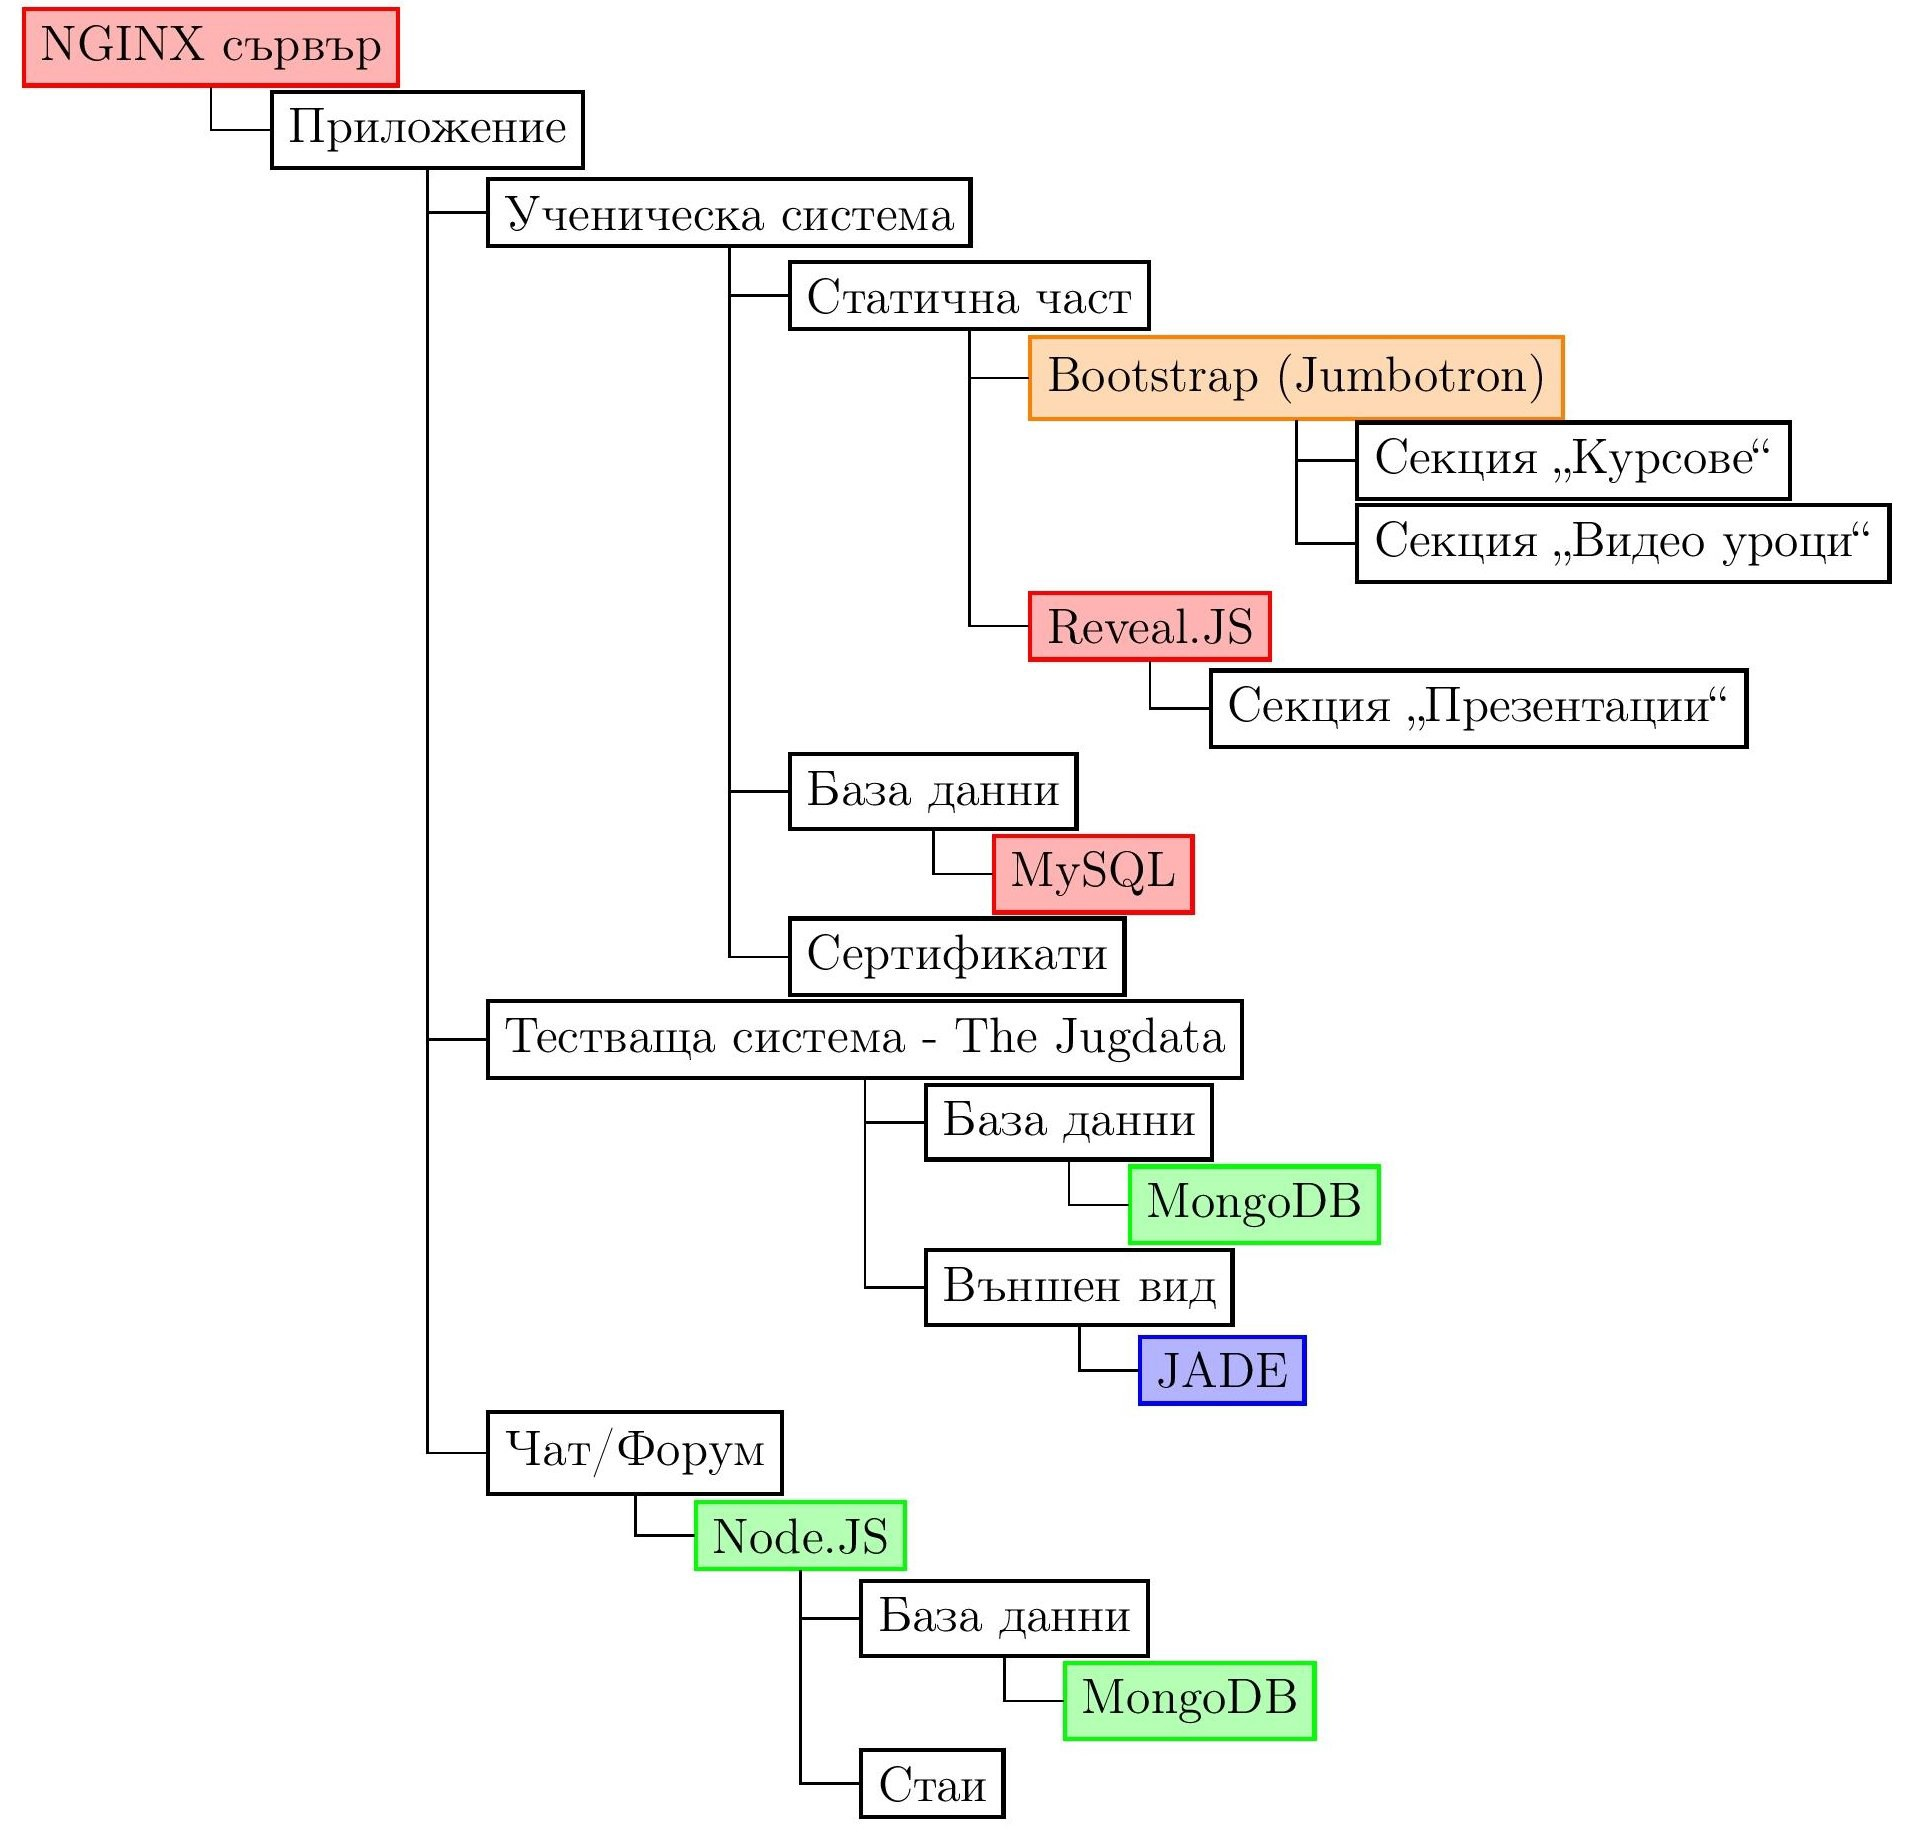
\includegraphics[width=0.75\textwidth]{arch.jpg}\\
	\section{Описание на приложението}
	Приложението е онлайн система и не се налага инсталиране на нещо по различно от браузър – системите не се нуждаят от приставки (като Flash Player и други).\\ 
	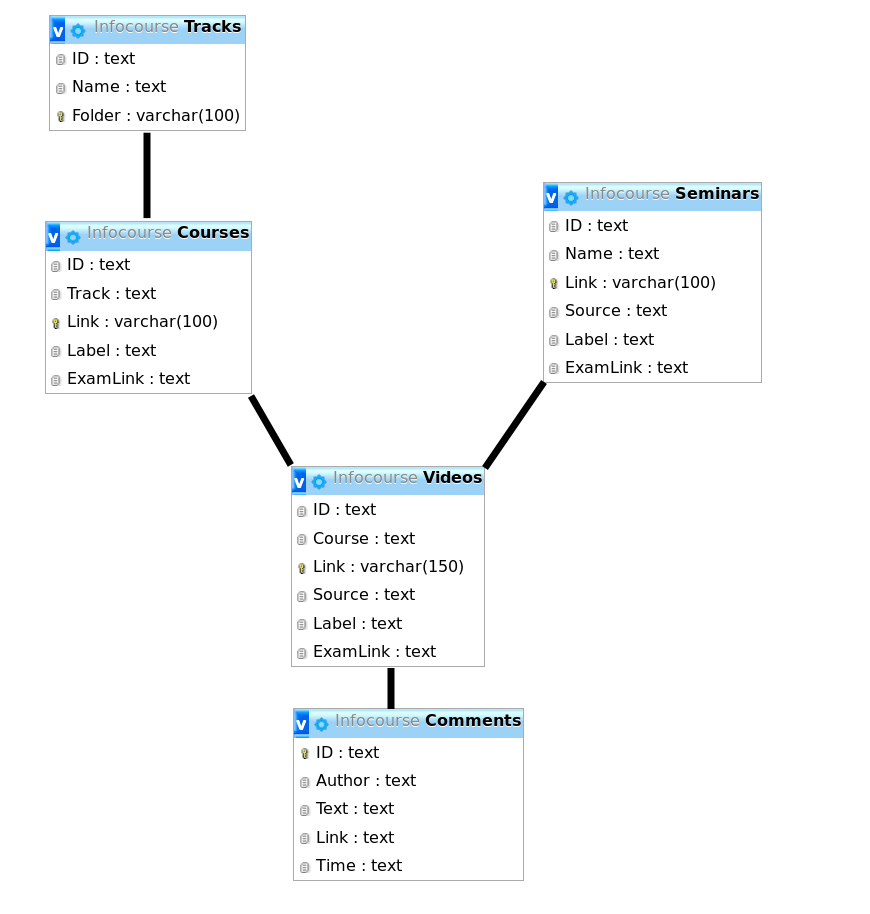
\includegraphics[width=0.75\textwidth]{mysql.png}\\
	\subsection{Използване на ученическата система}
	Тя има няколко начални опции – да се прегледа курс, да се прегледа семинар или да се прегледа информация за разработчиците и лекторите от бутона „About“ в горната част на сайта. Като, за да прегледате някой курс или семинар, трябва да кликнете върху съответния бутон „View video »“.\\
	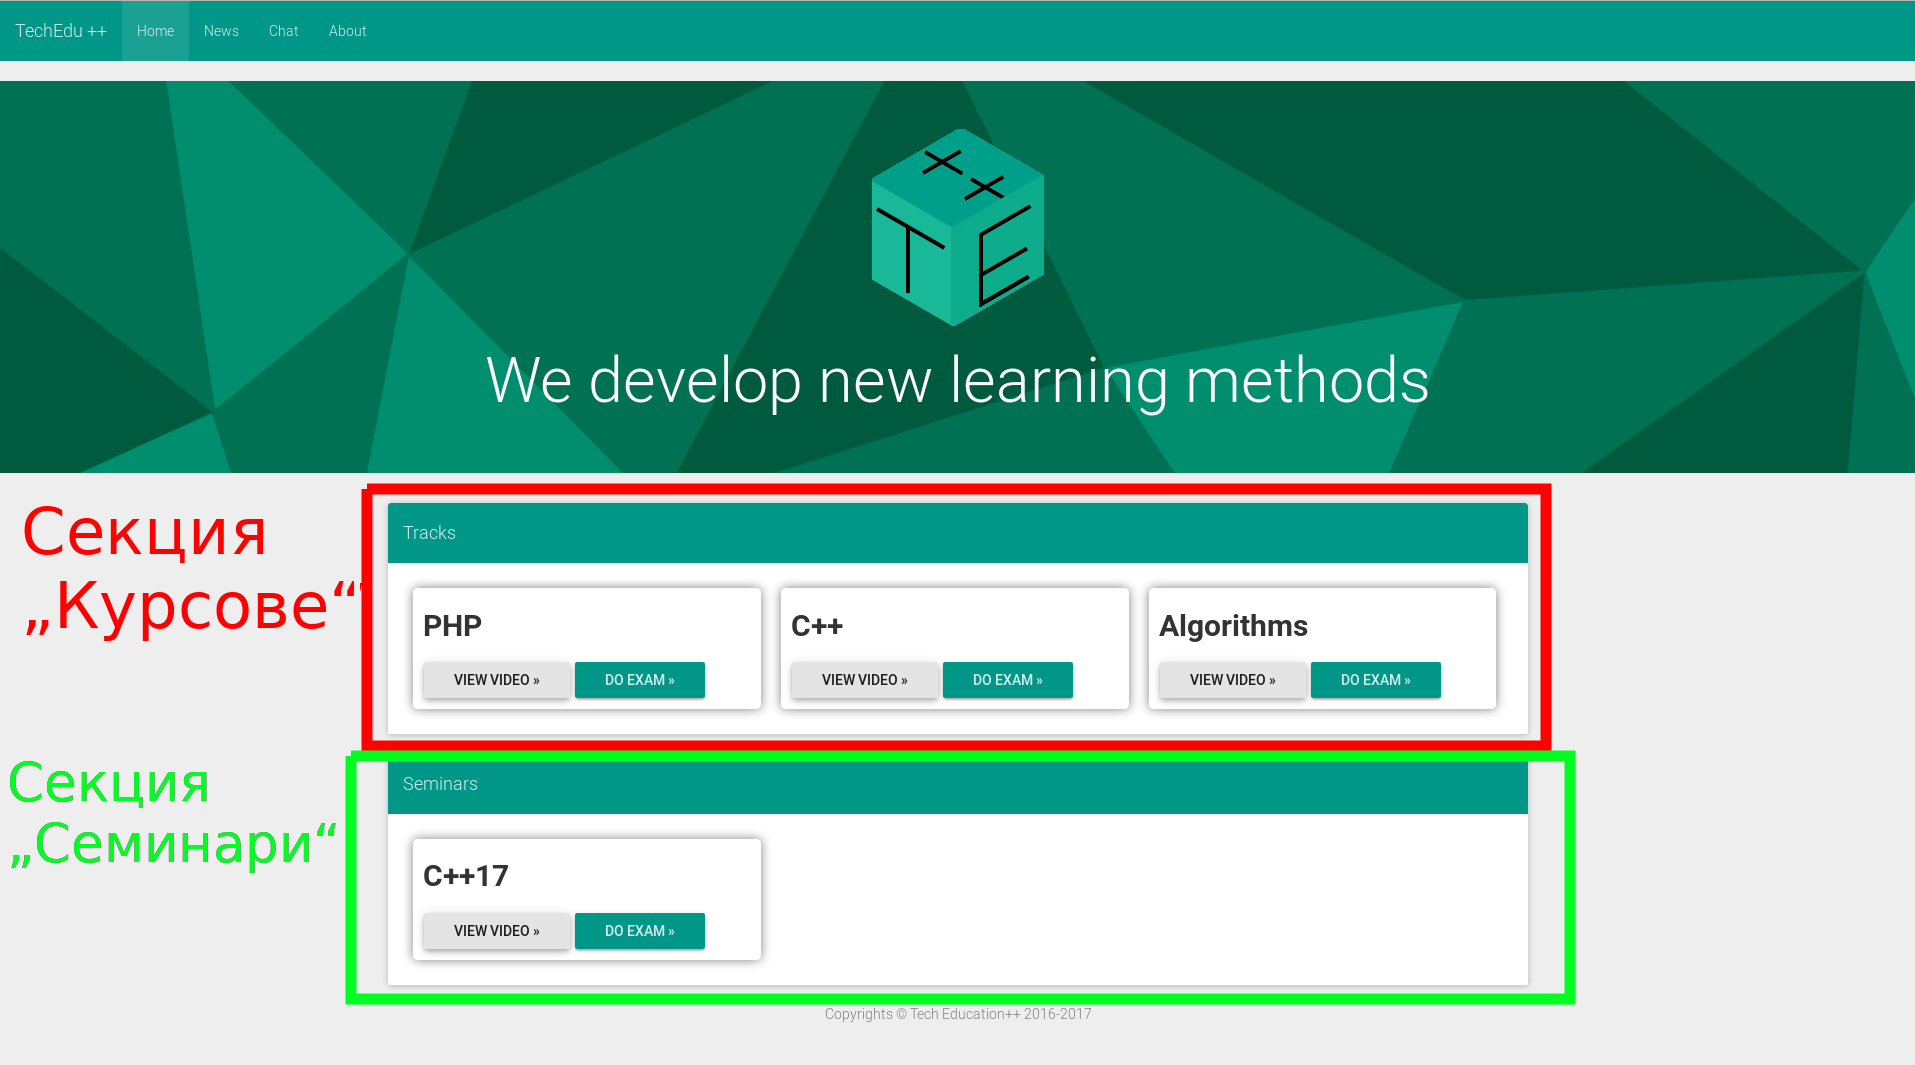
\includegraphics[width=1\textwidth]{track_view.png}\\
	\\При преглед на трак има множество курсове (например за начинаещи и напреднали), а всеки курс има множество озаглавени уроци и когато се кликне бутона „View video »“ се появява страница за съответното видео.\\
	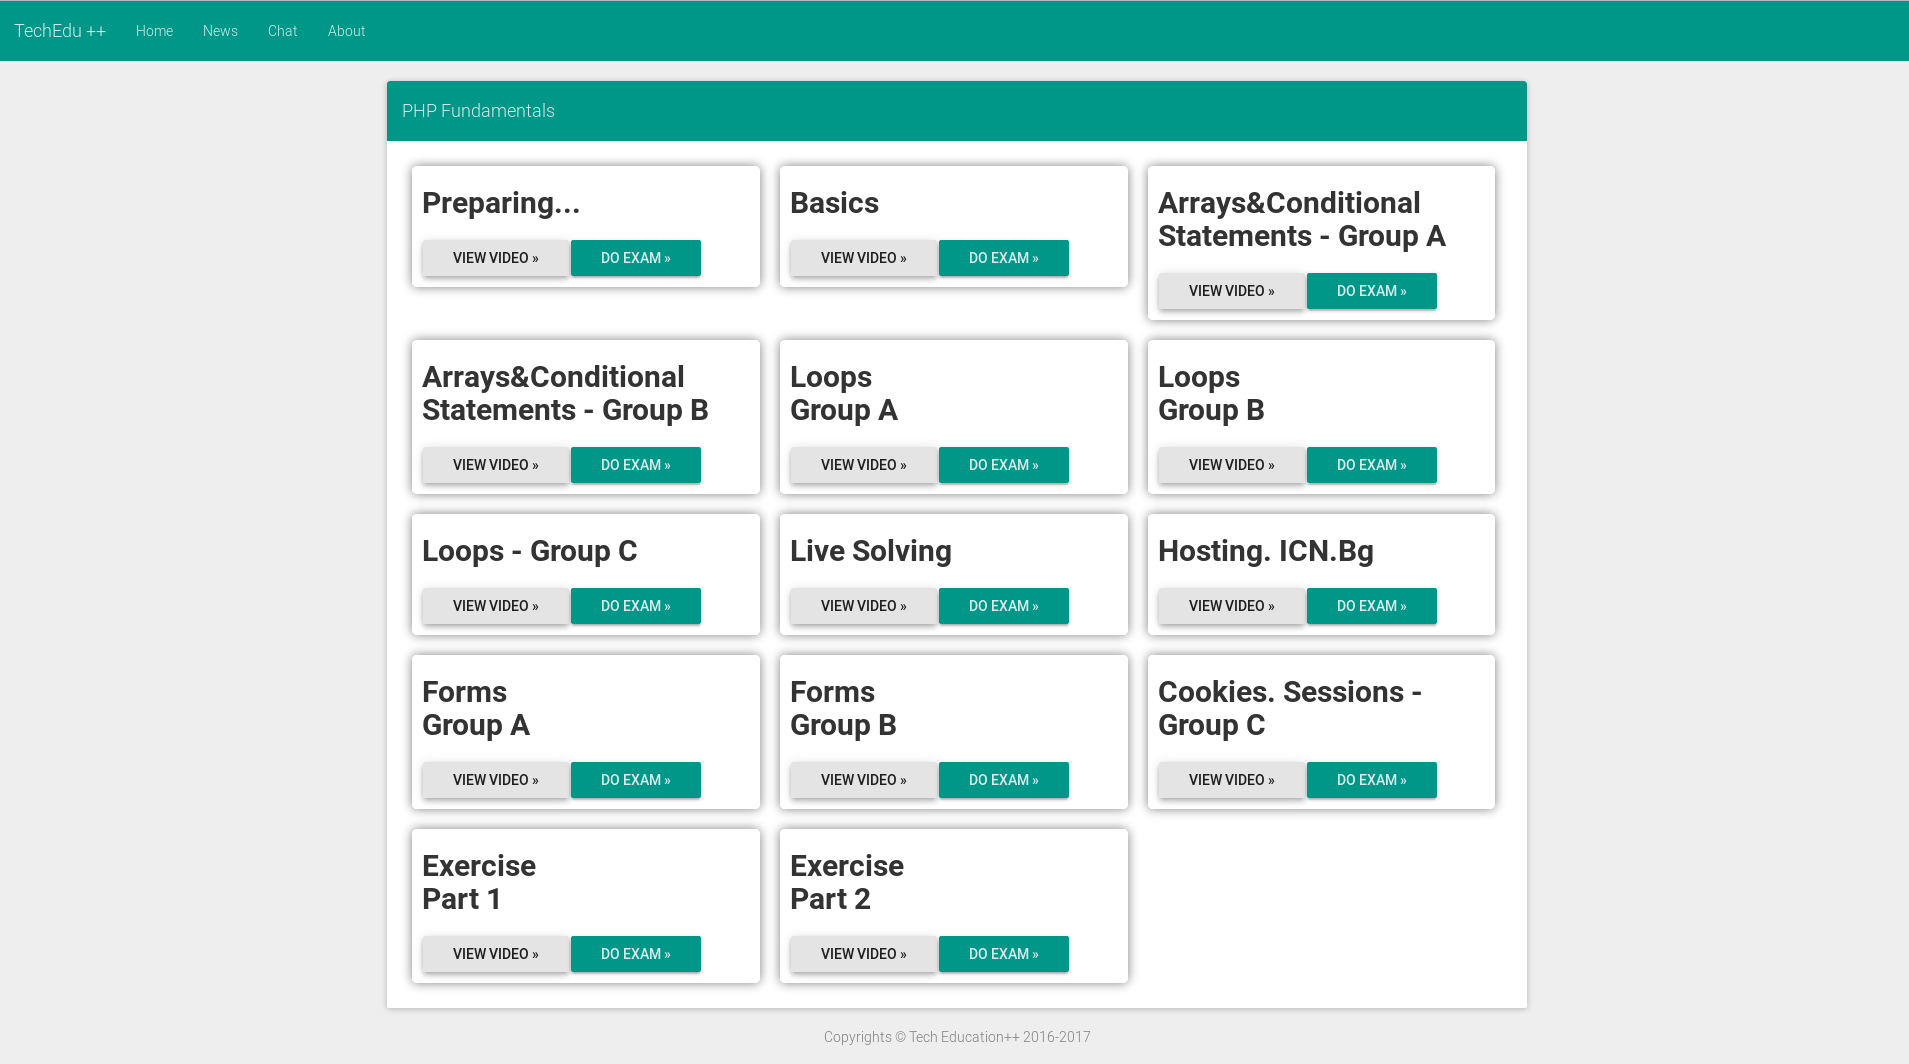
\includegraphics[width=1\textwidth]{view_details.png}\\
	\\За да се прегледате съответния видео урок, трябва да се натисне бутона „View video »“ за съответния урок и се появява вграден прозорец със съответното видео и опция за коментиране и преглед на коментарите към видеото.\\
	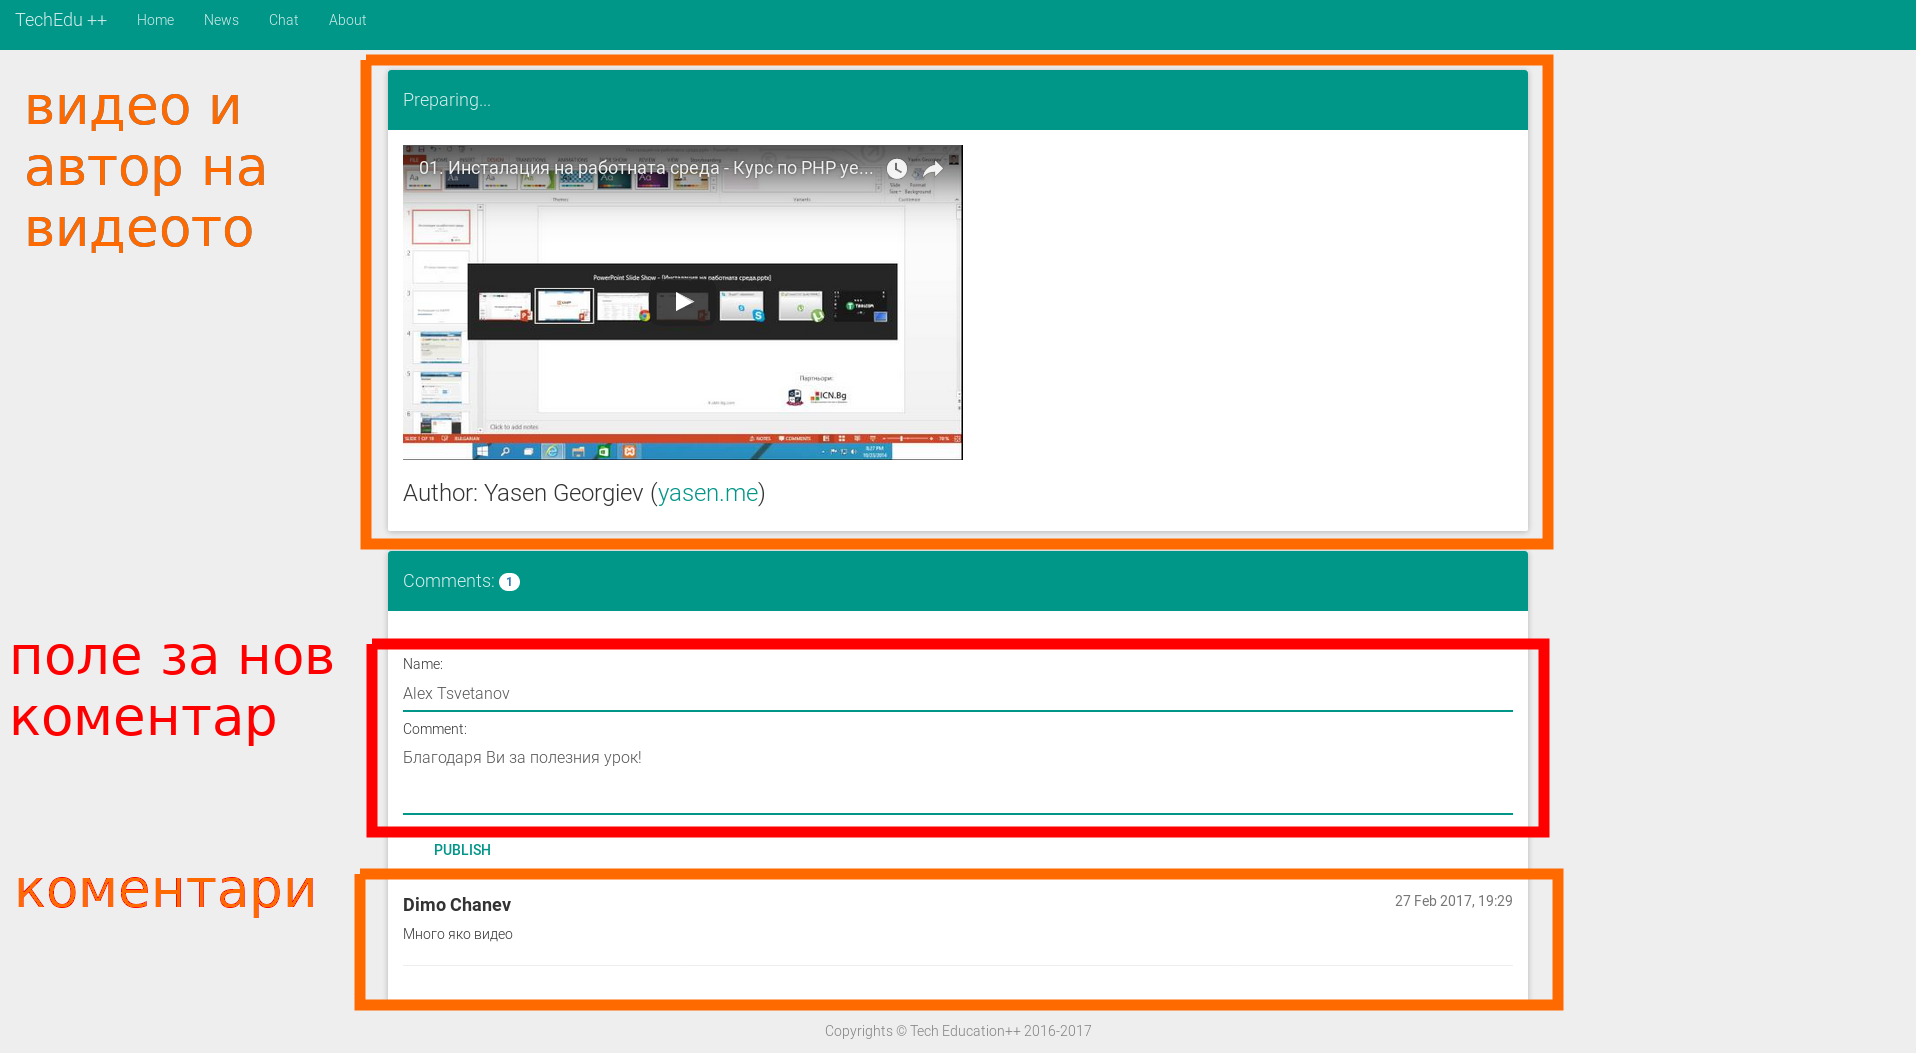
\includegraphics[width=1\textwidth]{video.png}\\
	\\При преглед на семинар директно ще се появи вграден прозорец със съответното видео.\\
	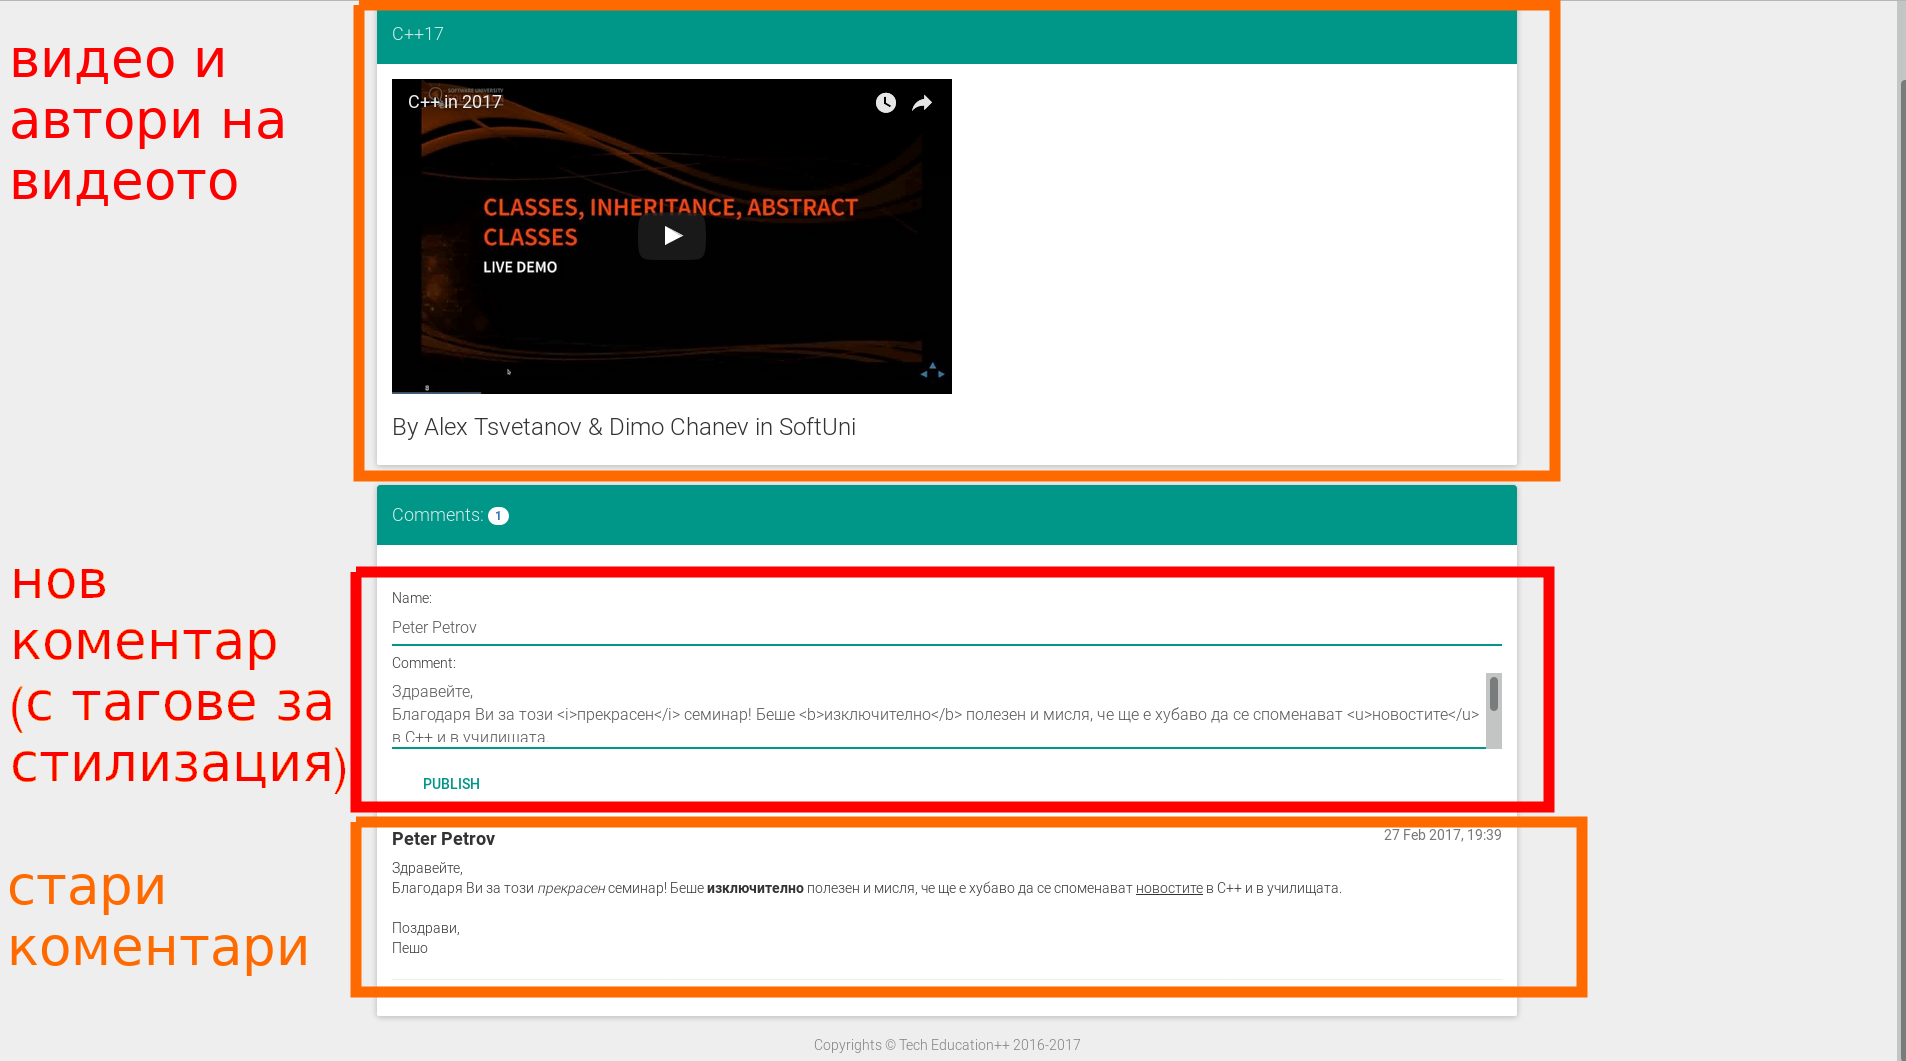
\includegraphics[width=1\textwidth]{seminar_video.png}\\
	\subsection{Използване на тестващата система}
	Началната ѝ страница също има няколко начални опции - управление на потребителя(register, login, logout) и участие във активните състезания.\\
  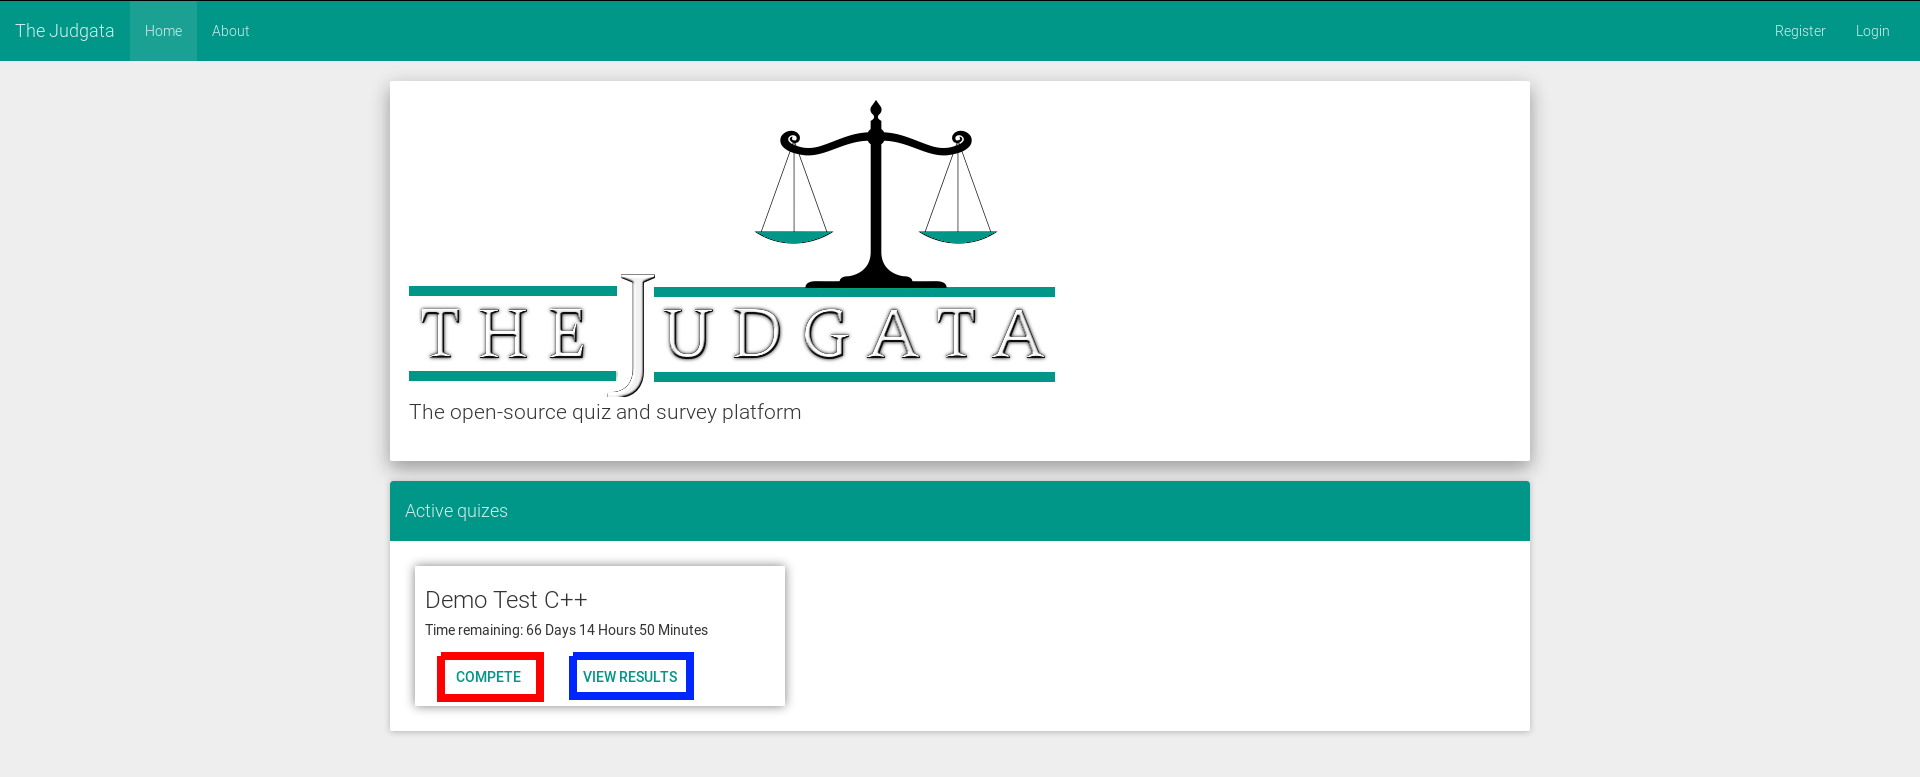
\includegraphics[width=1\textwidth]{judge_home.png}\\
	\\След като е избрано състезание(засега само практически задачи са поддържани) се вижда страницата за изпращане на решение.\\
	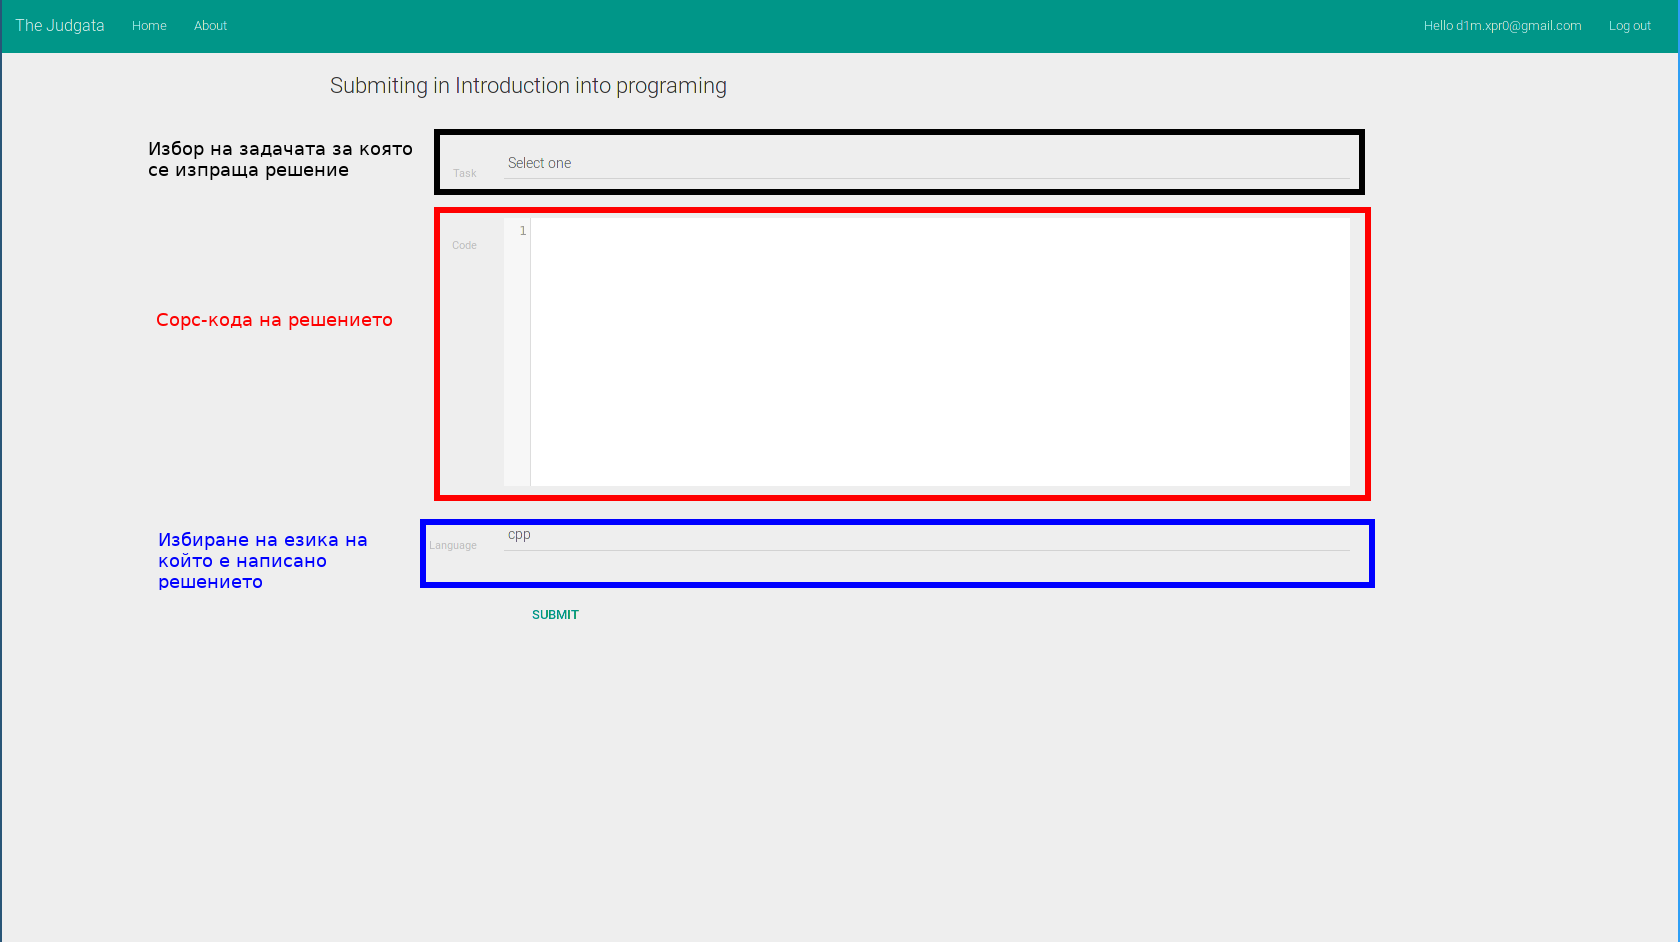
\includegraphics[width=1\textwidth]{judge_submi.png}\\
	\section{Още възможности на системите}
	Системите позволяват достъп на външни програми до публичната информация чрез т.н. APIs.
	\subsection{Линкове}
	Ученическата система се хоства на infocourse.SMG.bg \\
	Оценяващата система се хоства на judge.SMG.bg
	\section{Налични материали в платформата}
	\subsection{Училищна система}
	Училищната система постепенно се запълва с уроци! Вече имаме:
	\begin{itemize}
	  \item 49 видео урока за „PHP \& MySQL“, „C++“ и „Алгоритми“
	  %\item 1 семинар на тема „С++ през 2017“
	  %\item 5 новини, свързани с информатиката и информационните технологии
	  %\item 71 различни шеги за програмисти (за развлечение и освежаване на ума :D)
	  %\item 10 интересни факта за известни личности, свързани с ИИТ
	\end{itemize}
	%Уроците са изготвени от ученици от Правец и учители по информатика от София.
	\section{Заключение}
	Резултатът до момента е създаването на основата на образователно-информационна платформа, която да може да се усъвършенства и обновява, за да бъде в крак с времето и технологиите. 
	Бъдещото развитие включва:
	\begin{itemize}
		\item добавяне на система от знания по други актуални програмни езици като JavaScript, TypeScript, Java, Python и т.н.
		\item популяризиране на проекта сред учащите се (системата вече се използва от наши съученици в СМГ)
		\item разширяване на кръга от контакти с действащи фирми
	\end{itemize}
\end{document}
